\documentclass{scrartcl}
\usepackage[margin=3cm]{geometry}
\usepackage{amsmath}
\usepackage{amssymb}
\usepackage{amsthm}
\usepackage{blindtext}
\usepackage{datetime}
\usepackage{fontspec}
\usepackage{float}
\usepackage{graphicx}
\usepackage{kotex}
\usepackage[lighttt]{lmodern}
\usepackage{listings}
\usepackage{mathrsfs}
\usepackage{mathtools}
\usepackage{pgf,tikz,pgfplots}

\pgfplotsset{compat=1.15}
\usetikzlibrary{arrows}
\newtheorem{theorem}{Theorem}

\lstset{
  numbers=none, frame=single, showspaces=false,
  showstringspaces=false, showtabs=false, breaklines=true, showlines=true,
  breakatwhitespace=true, basicstyle=\ttfamily, keywordstyle=\bfseries, basewidth=0.5em
}

\setmainhangulfont{Noto Serif CJK KR}[
  UprightFont=* Light, BoldFont=* Bold,
  Script=Hangul, Language=Korean, AutoFakeSlant,
]
\setsanshangulfont{Noto Sans CJK KR}[
  UprightFont=* DemiLight, BoldFont=* Medium,
  Script=Hangul, Language=Korean
]
\setmathhangulfont{Noto Sans CJK KR}[
  SizeFeatures={
    {Size=-6,  Font=* Medium},
    {Size=6-9, Font=*},
    {Size=9-,  Font=* DemiLight},
  },
  Script=Hangul, Language=Korean
]
\title{디지털시스템설계 Lab 5}
\author{손량(20220323)}
\date{Last compiled on: \today, \currenttime}

\newcommand{\un}[1]{\ensuremath{\ \mathrm{#1}}}

\begin{document}
\maketitle

\section{개요}
현대적인 컴퓨터의 기반이 되는 ALU와 flip-flop을 verilog로 구현해 보고, 시물레이션과 실험을 통해 작동을 확인한다.

\section{이론적 배경}
\subsection{ALU}
ALU는 입력이 주어졌을 때 산술, 논리 연산을 수행하는 회로이다.
입력에 따라 수행할 연산을 골라서 operand끼리 연산을 수행한다.

\subsection{비동기 회로와 동기 회로}
클럭 등의 신호를 이용하여 내부의 구성 요소들을 동기화하는 회로를 동기 회로, 그렇지 않은 회로를 비동기 회로라고 부른다.
비동기 회로의 예시로는 Combinational logic, 클럭과 상관없이 동작하는 회로가 있다.
이번 lab 5에서 다루는 회로 중 latch는 비동기 회로, flip-flop은 동기 회로에 해당한다.

\subsection{JK Latch}
가장 기본적인 latch인 SR latch는 forbidden state가 존재한다는 단점이 있다.
JK latch는 SR latch에 게이트를 추가하여 forbidden state가 일어나지 않도록 한다.
SR latch에서 forbidden state에 해당하는 입력은 JK latch에서는 저장된 비트를 반전시키는 데에 사용한다.

JK latch에 클럭 신호를 통한 동기화를 추가하면 JK flip-flop을 만들 수 있다.

\subsection{Master-Slave JK Flip-Flop}
Master-slave JK flip-flop은 SR 래치 두 개를 연결해 만든 flip-flop 회로이다.
이름이 의미하듯 master latch와 slave latch가 존재한다.
클럭이 1인 동안에는 master latch가 활성화되어 입력을 저장하고, 0인 동안에는 slave latch가 활성화되어 master latch의 출력을 저장하게 된다.

클럭이 0인 동안에는 slave latch에 들어가는 입력이 일정하기 때문에 상관없지만, 클럭이 1인 동안에는 계속 입력을 받으므로 master latch에 글리치로 인해 잠깐 입력이 생기면 글리치를 정상적인 신호로 인식한다는 문제점이 존재한다.
이를 1's catch라고 부르고, edge-trigger 회로를 사용하여 해결하는 방법이 있다.

\section{실험 준비}
\subsection{ALU}
ALU의 전체적인 회로도는 다음과 같다.
\begin{figure}[H]
  \centering
  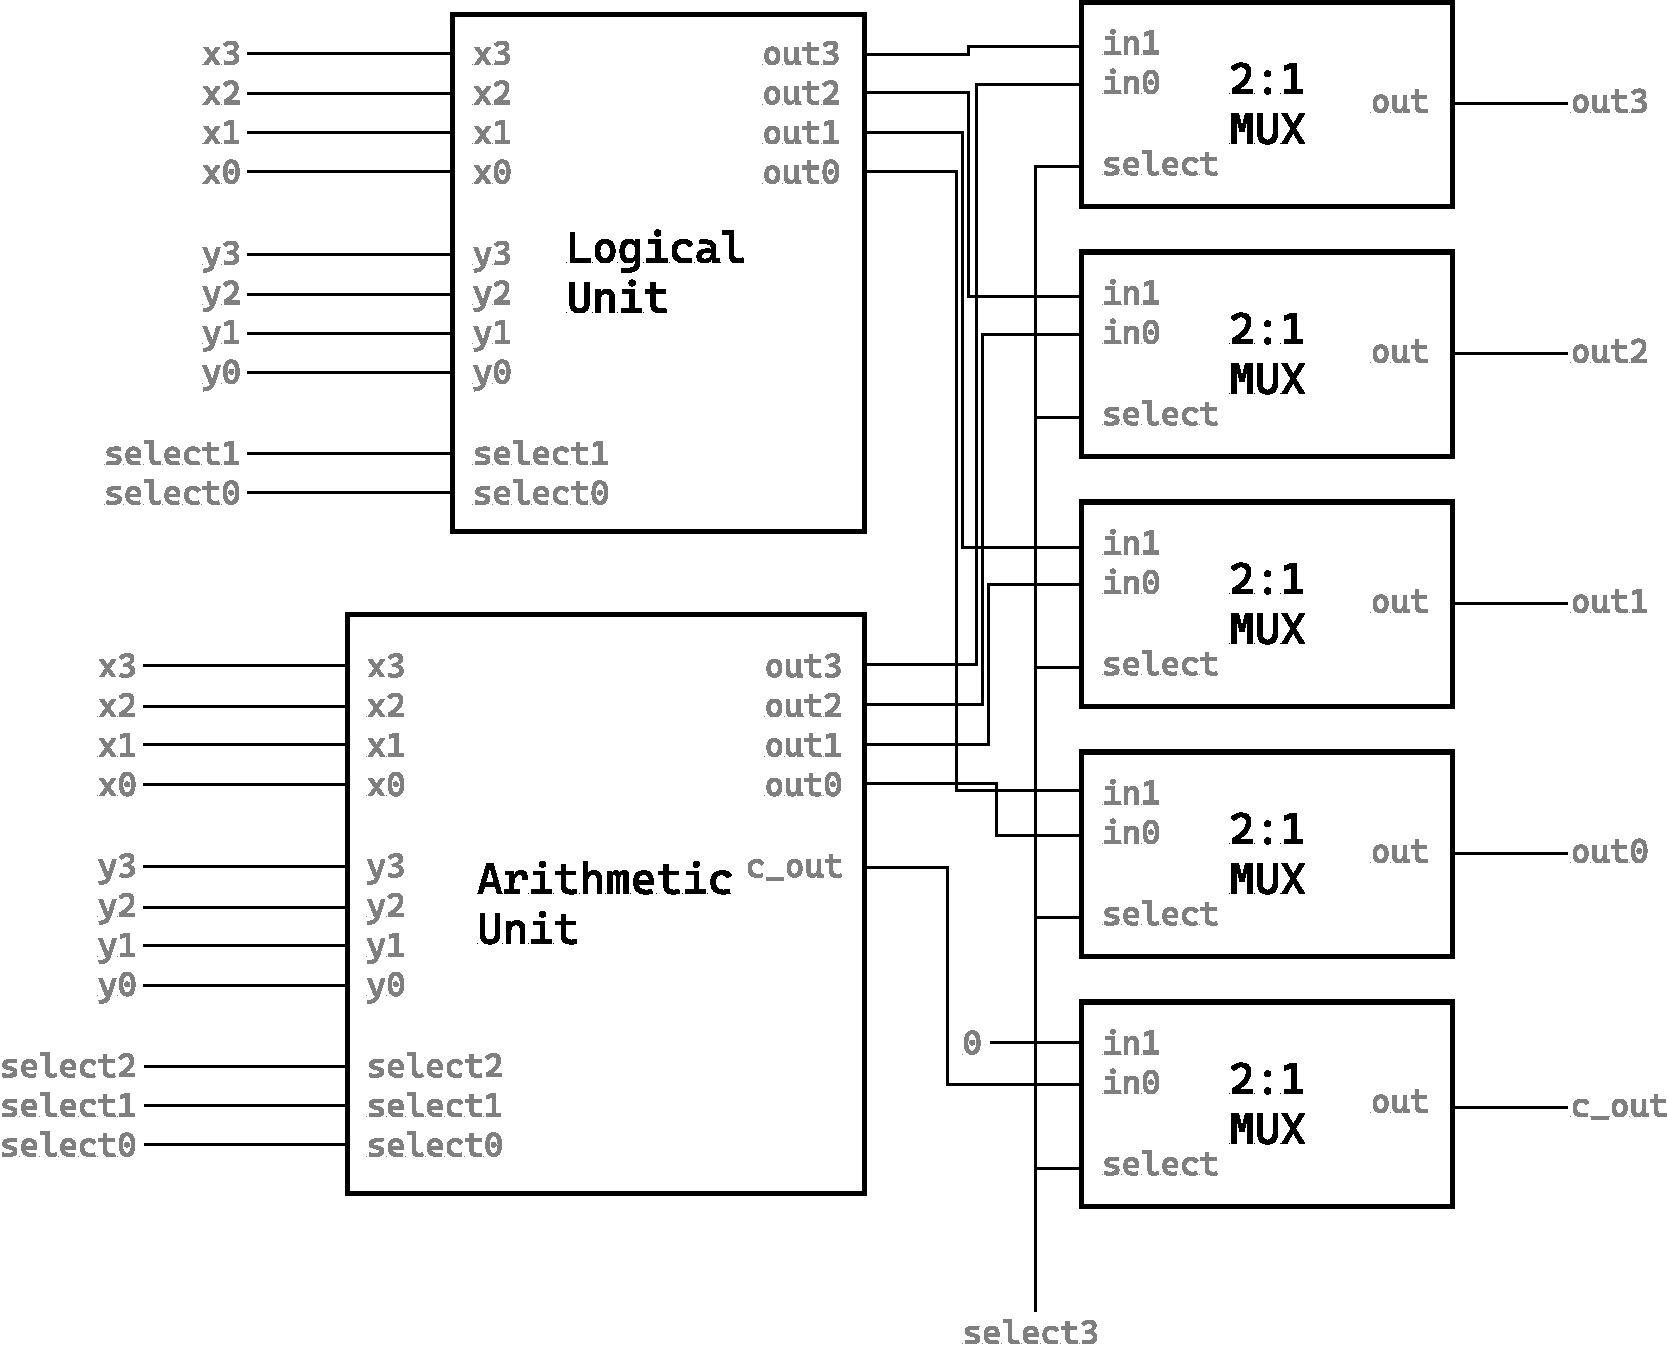
\includegraphics[width=0.9\linewidth]{alu_schematic.pdf}
\end{figure}

Arithmetic unit의 회로도는 다음과 같다.
\begin{figure}[H]
  \centering
  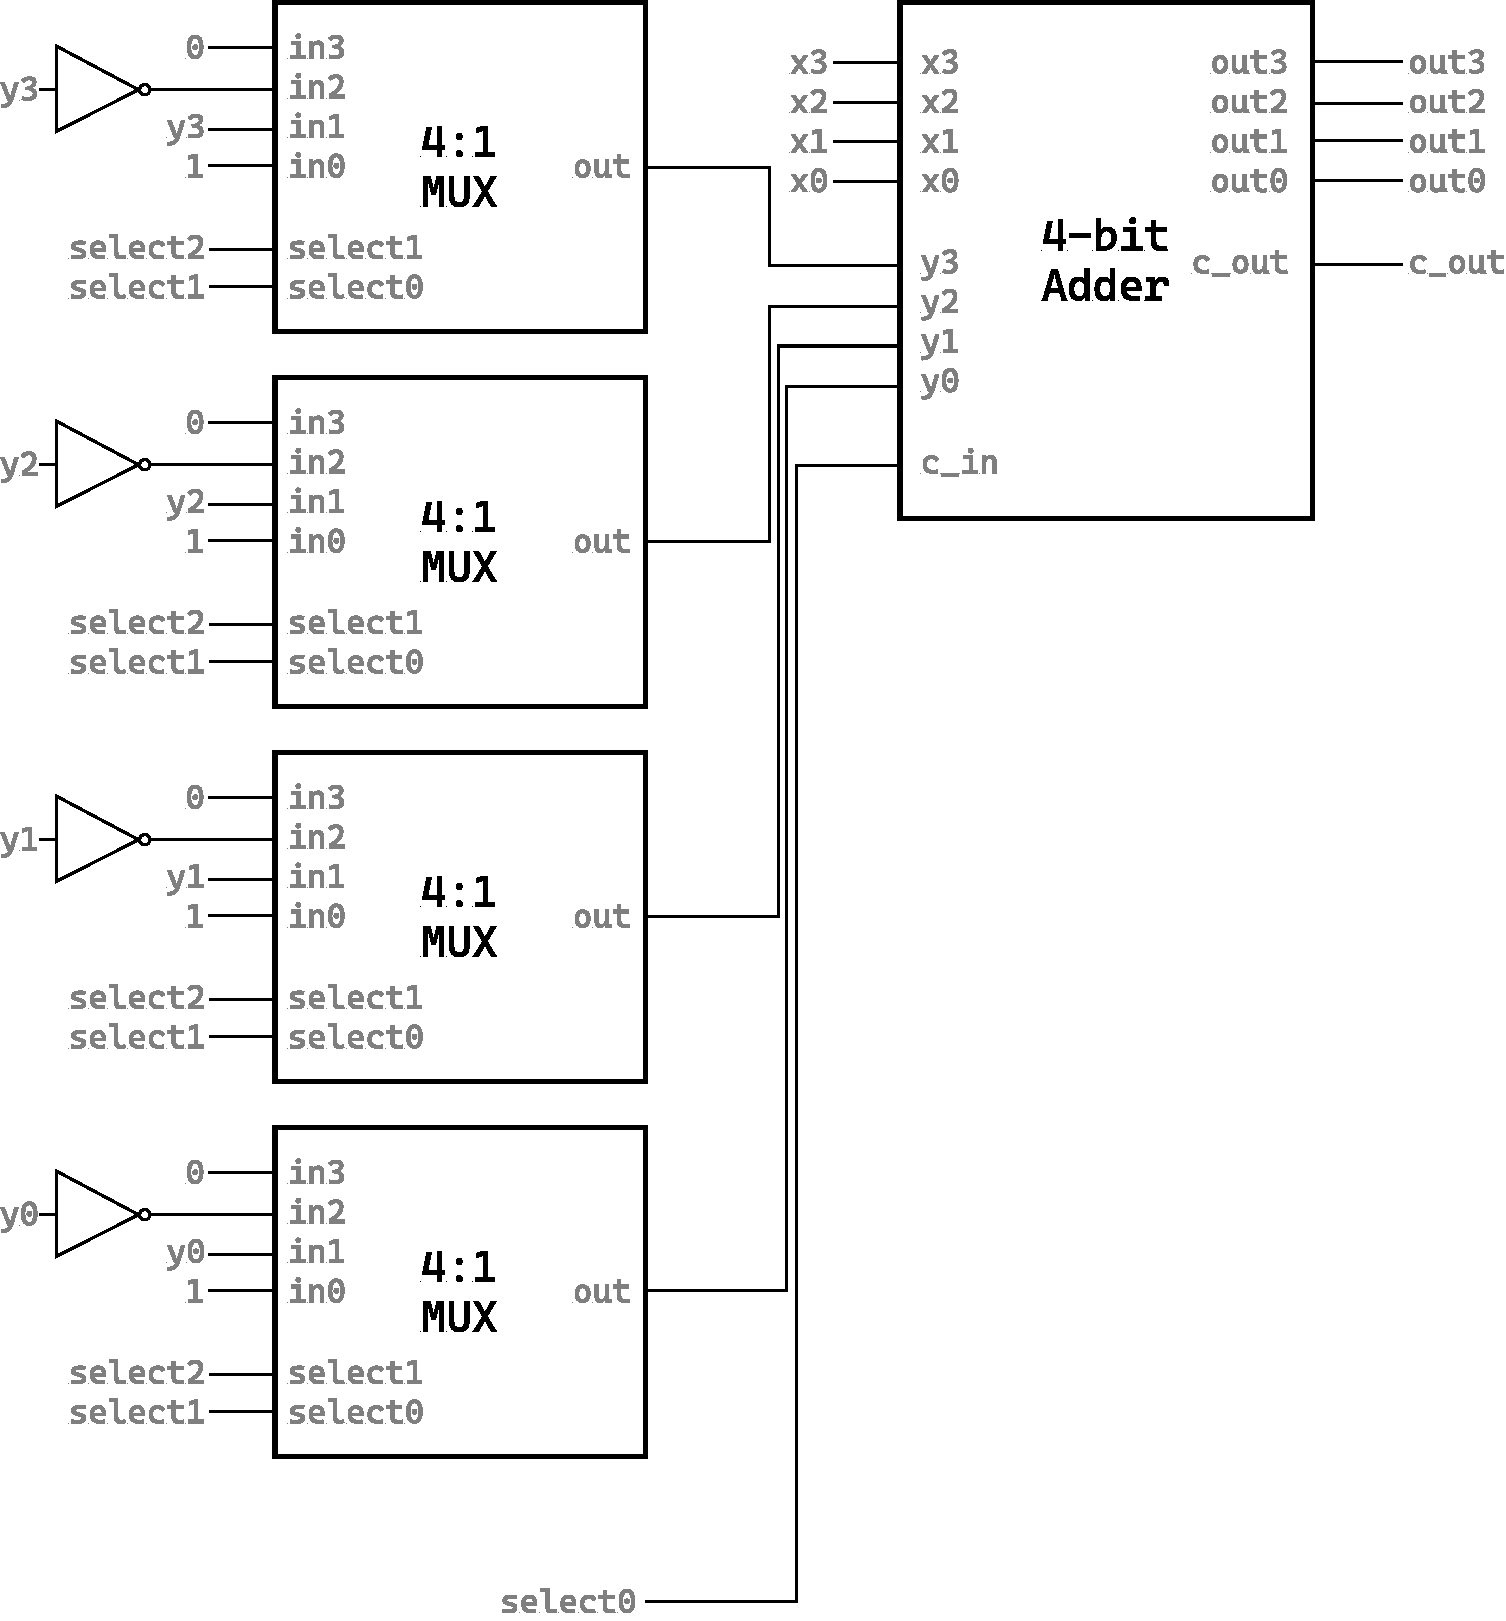
\includegraphics[width=0.9\linewidth]{arith_unit_schematic.pdf}
\end{figure}

Logical unit의 회로도는 다음과 같다.
\begin{figure}[H]
  \centering
  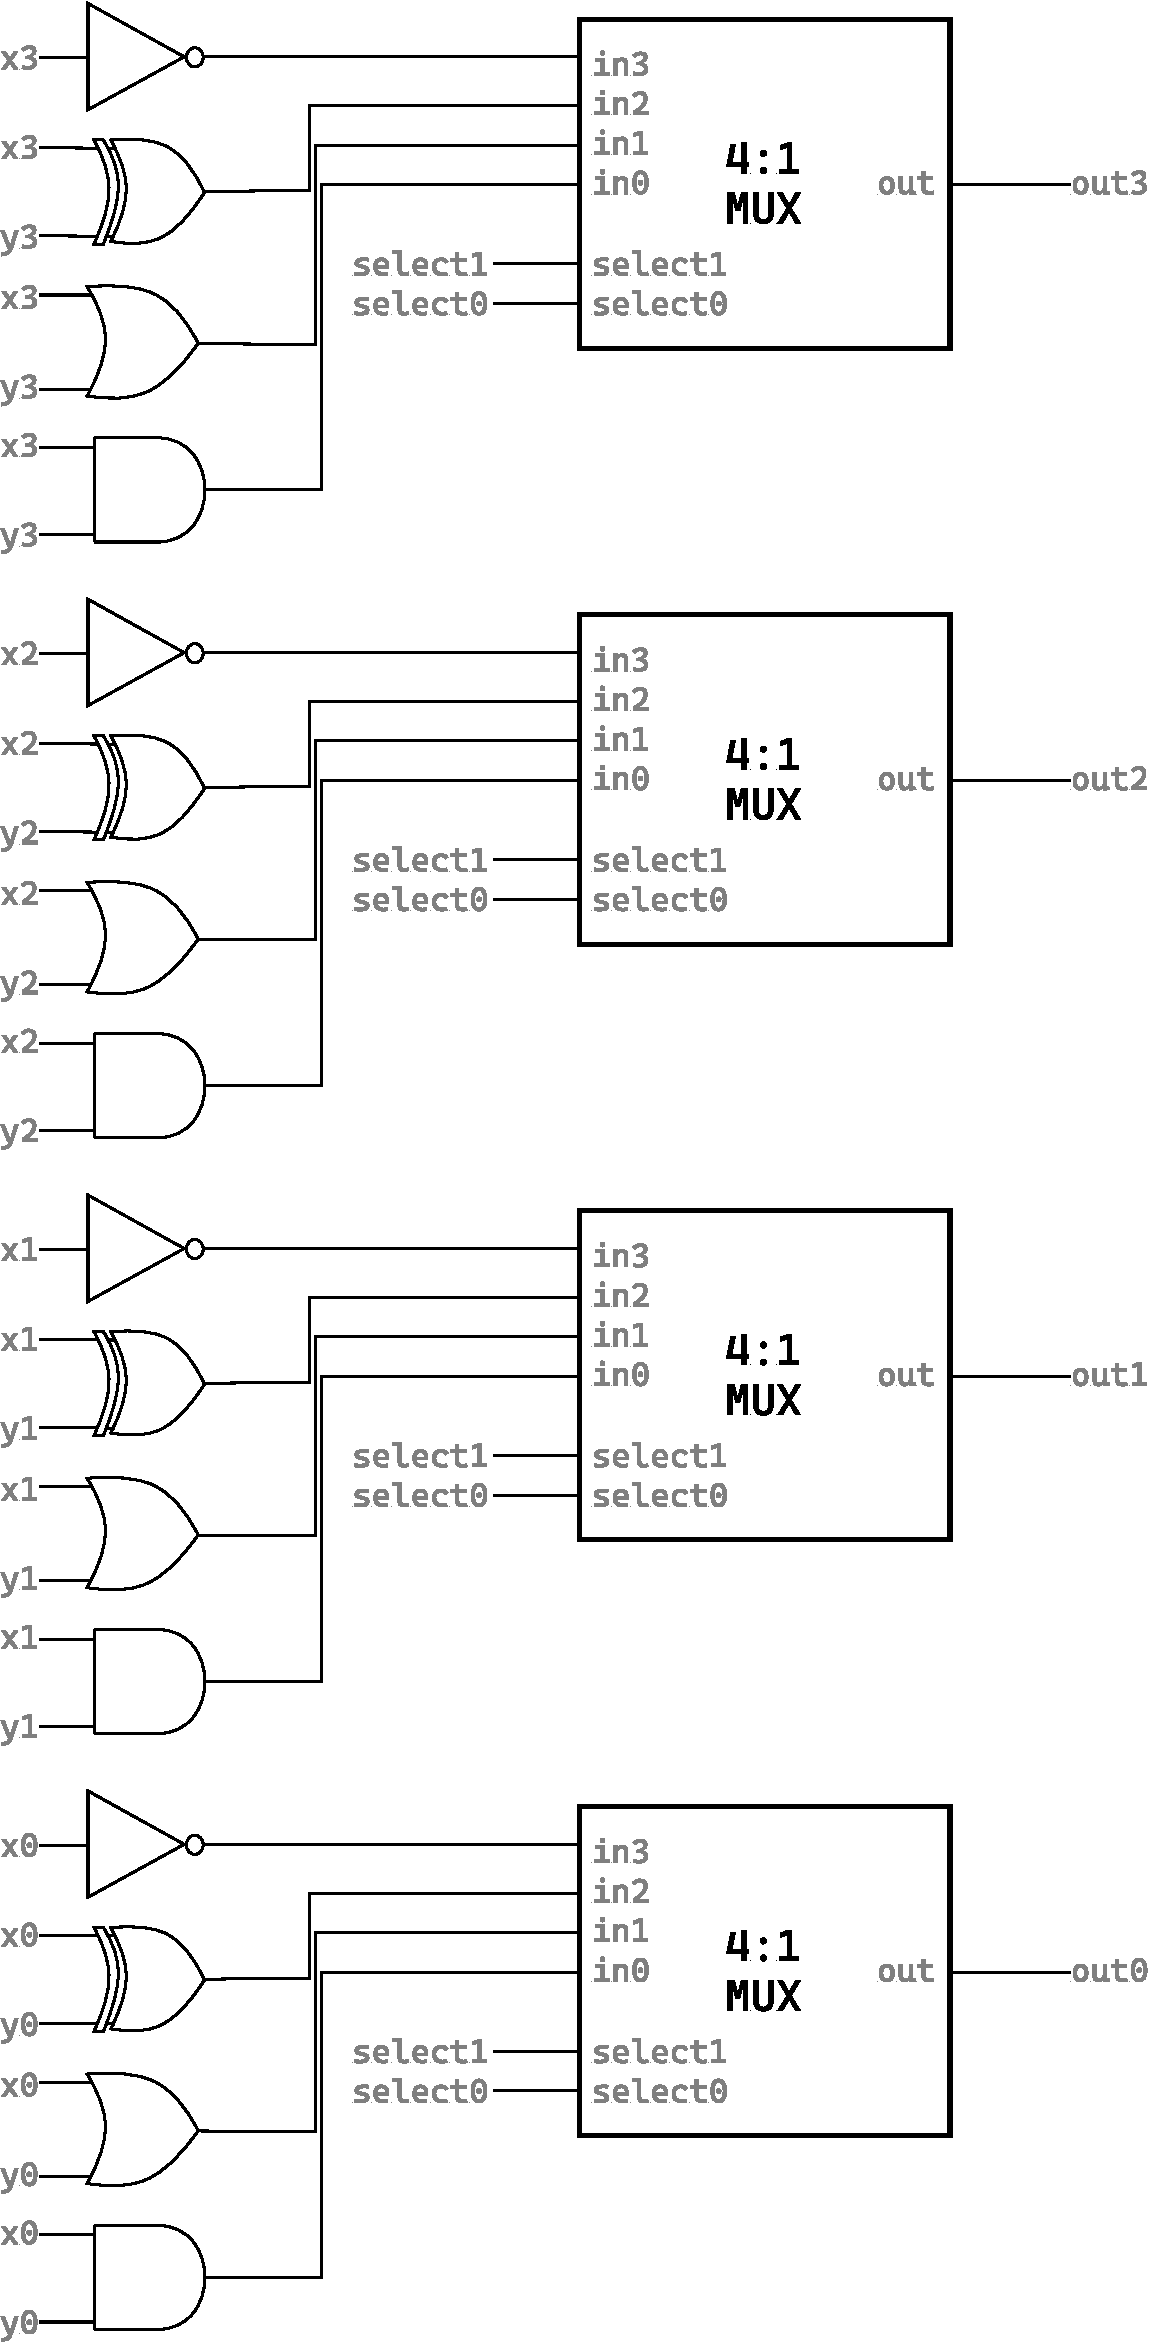
\includegraphics[width=0.7\linewidth]{logical_unit_schematic.pdf}
\end{figure}

\subsection{Master-Slave JK Flip-Flop}
SR latch의 회로도는 다음과 같다.
\begin{figure}[H]
  \centering
  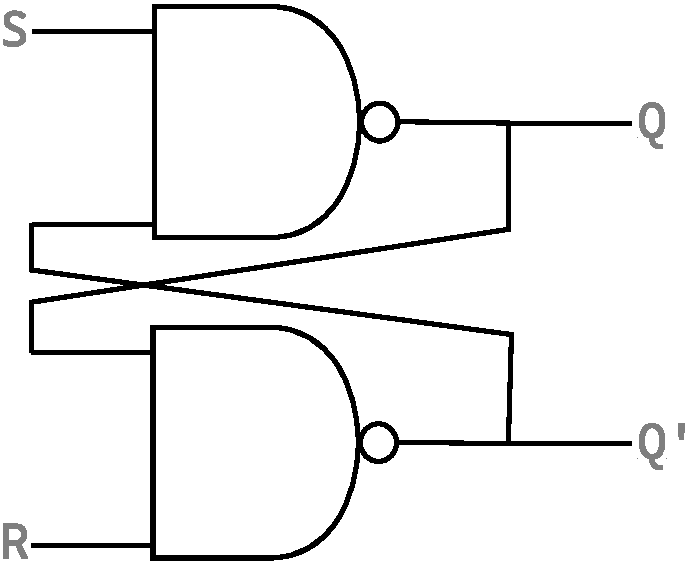
\includegraphics[width=0.4\linewidth]{sr_schematic.pdf}
\end{figure}

Negative reset master-slave JK flip-flop의 회로도는 다음과 같다.
\begin{figure}[H]
  \centering
  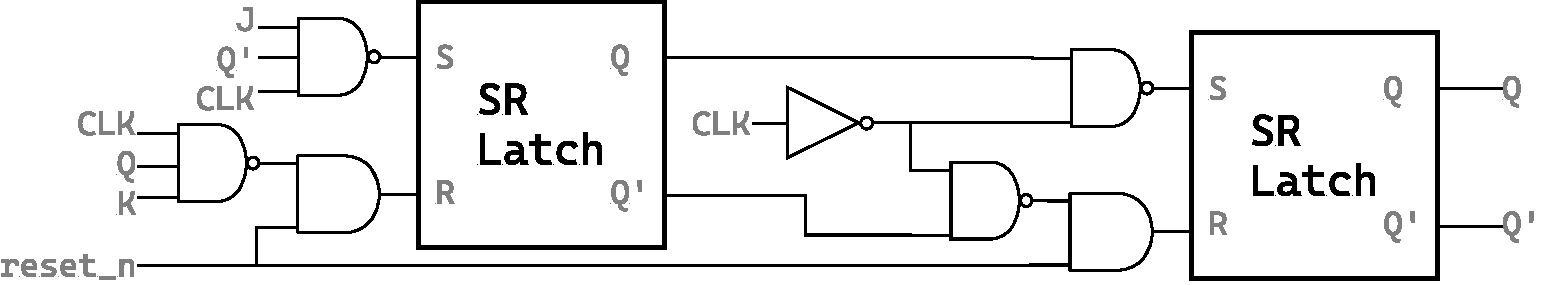
\includegraphics[width=0.9\linewidth]{jkff_schematic.pdf}
\end{figure}

이 회로도의 SR latch는 \(S = R = 0\) 입력이 금지되어 있고, \(S = R = 1\) 입력 직후에 \(S = R = 0\)을 입력한다면 racing 현상과 같은 비정상적인 동작을 할 수 있다.
반면 master-slave flip-flop의 경우 SR latch에 게이트와 클럭을 추가함으로써 \(S = R = 0\)과 같은 금지된 입력이 들어가지 못하도록 한다.
하지만 master-slave flip-flop의 설계에서 클럭이 1인 동안에는 master latch가 입력을 계속 받는 상태이기 때문에 글리치로 생긴 입력 값이 회로 동작에 영향을 끼치는, 1's catch가 일어날 수 있다는 단점은 SR latch와 마찬가지로 해결하지 못한다.

\section{실험 결과}
\subsection{\texttt{lab5\_1.v} -- ALU 구현}
화로도는 다음과 같다.
\begin{figure}[H]
  \centering
  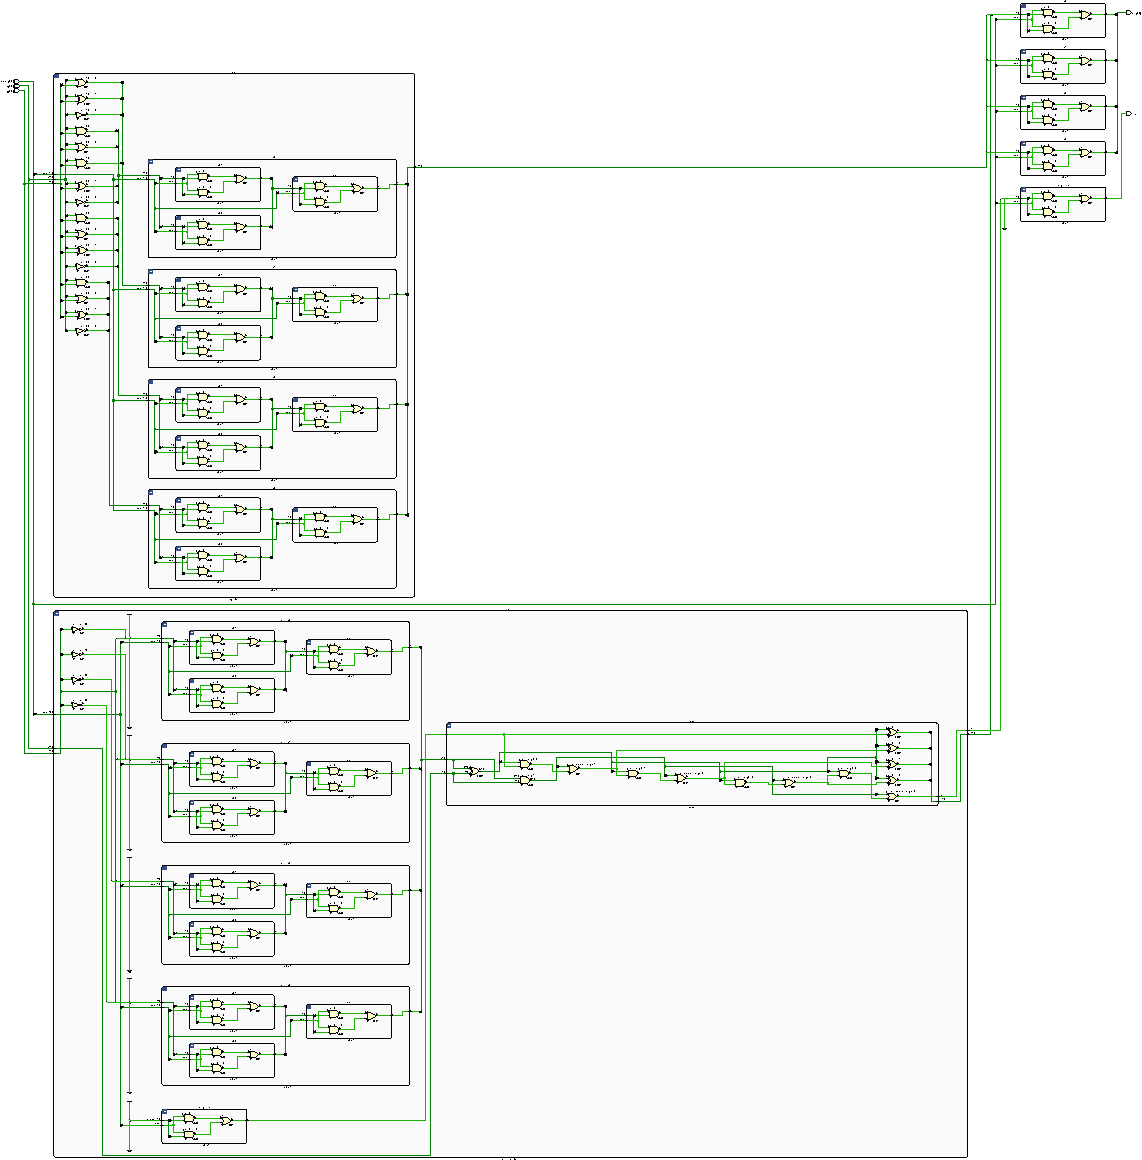
\includegraphics[width=0.9\linewidth]{lab5_1_schematic_expanded-crop.pdf}
\end{figure}
테스트벤치 실행 결과 다음 파형을 얻을 수 있었다.
\begin{figure}[H]
  \centering
  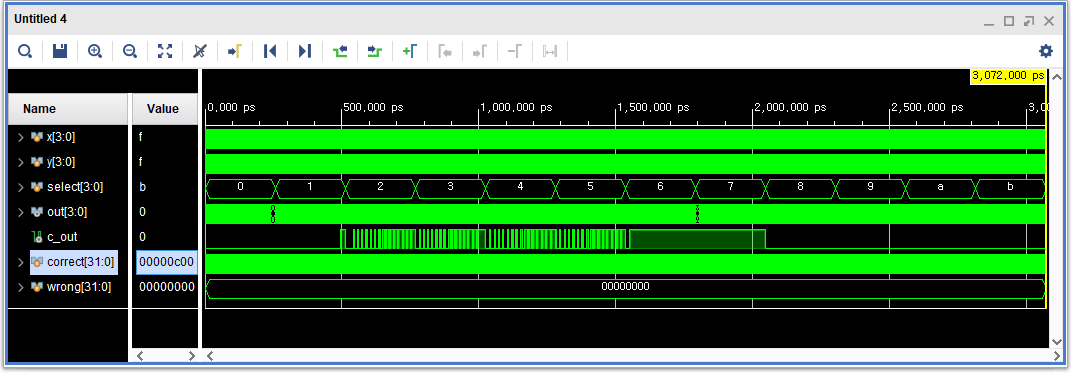
\includegraphics[width=0.9\linewidth]{lab5_1_waveform.png}
\end{figure}

\subsubsection{FPGA 실험 결과}
다음은 FPGA에서 코드를 실행한 결과들이다.
\(x = 13, y = 6\) 입력을 넣었고, \texttt{sel} 입력을 0부터 11까지 바꿔가며 실행한 결과는 다음과 같다.
\begin{figure}[H]
  \centering
  \begin{minipage}{0.45\linewidth}
    \centering
    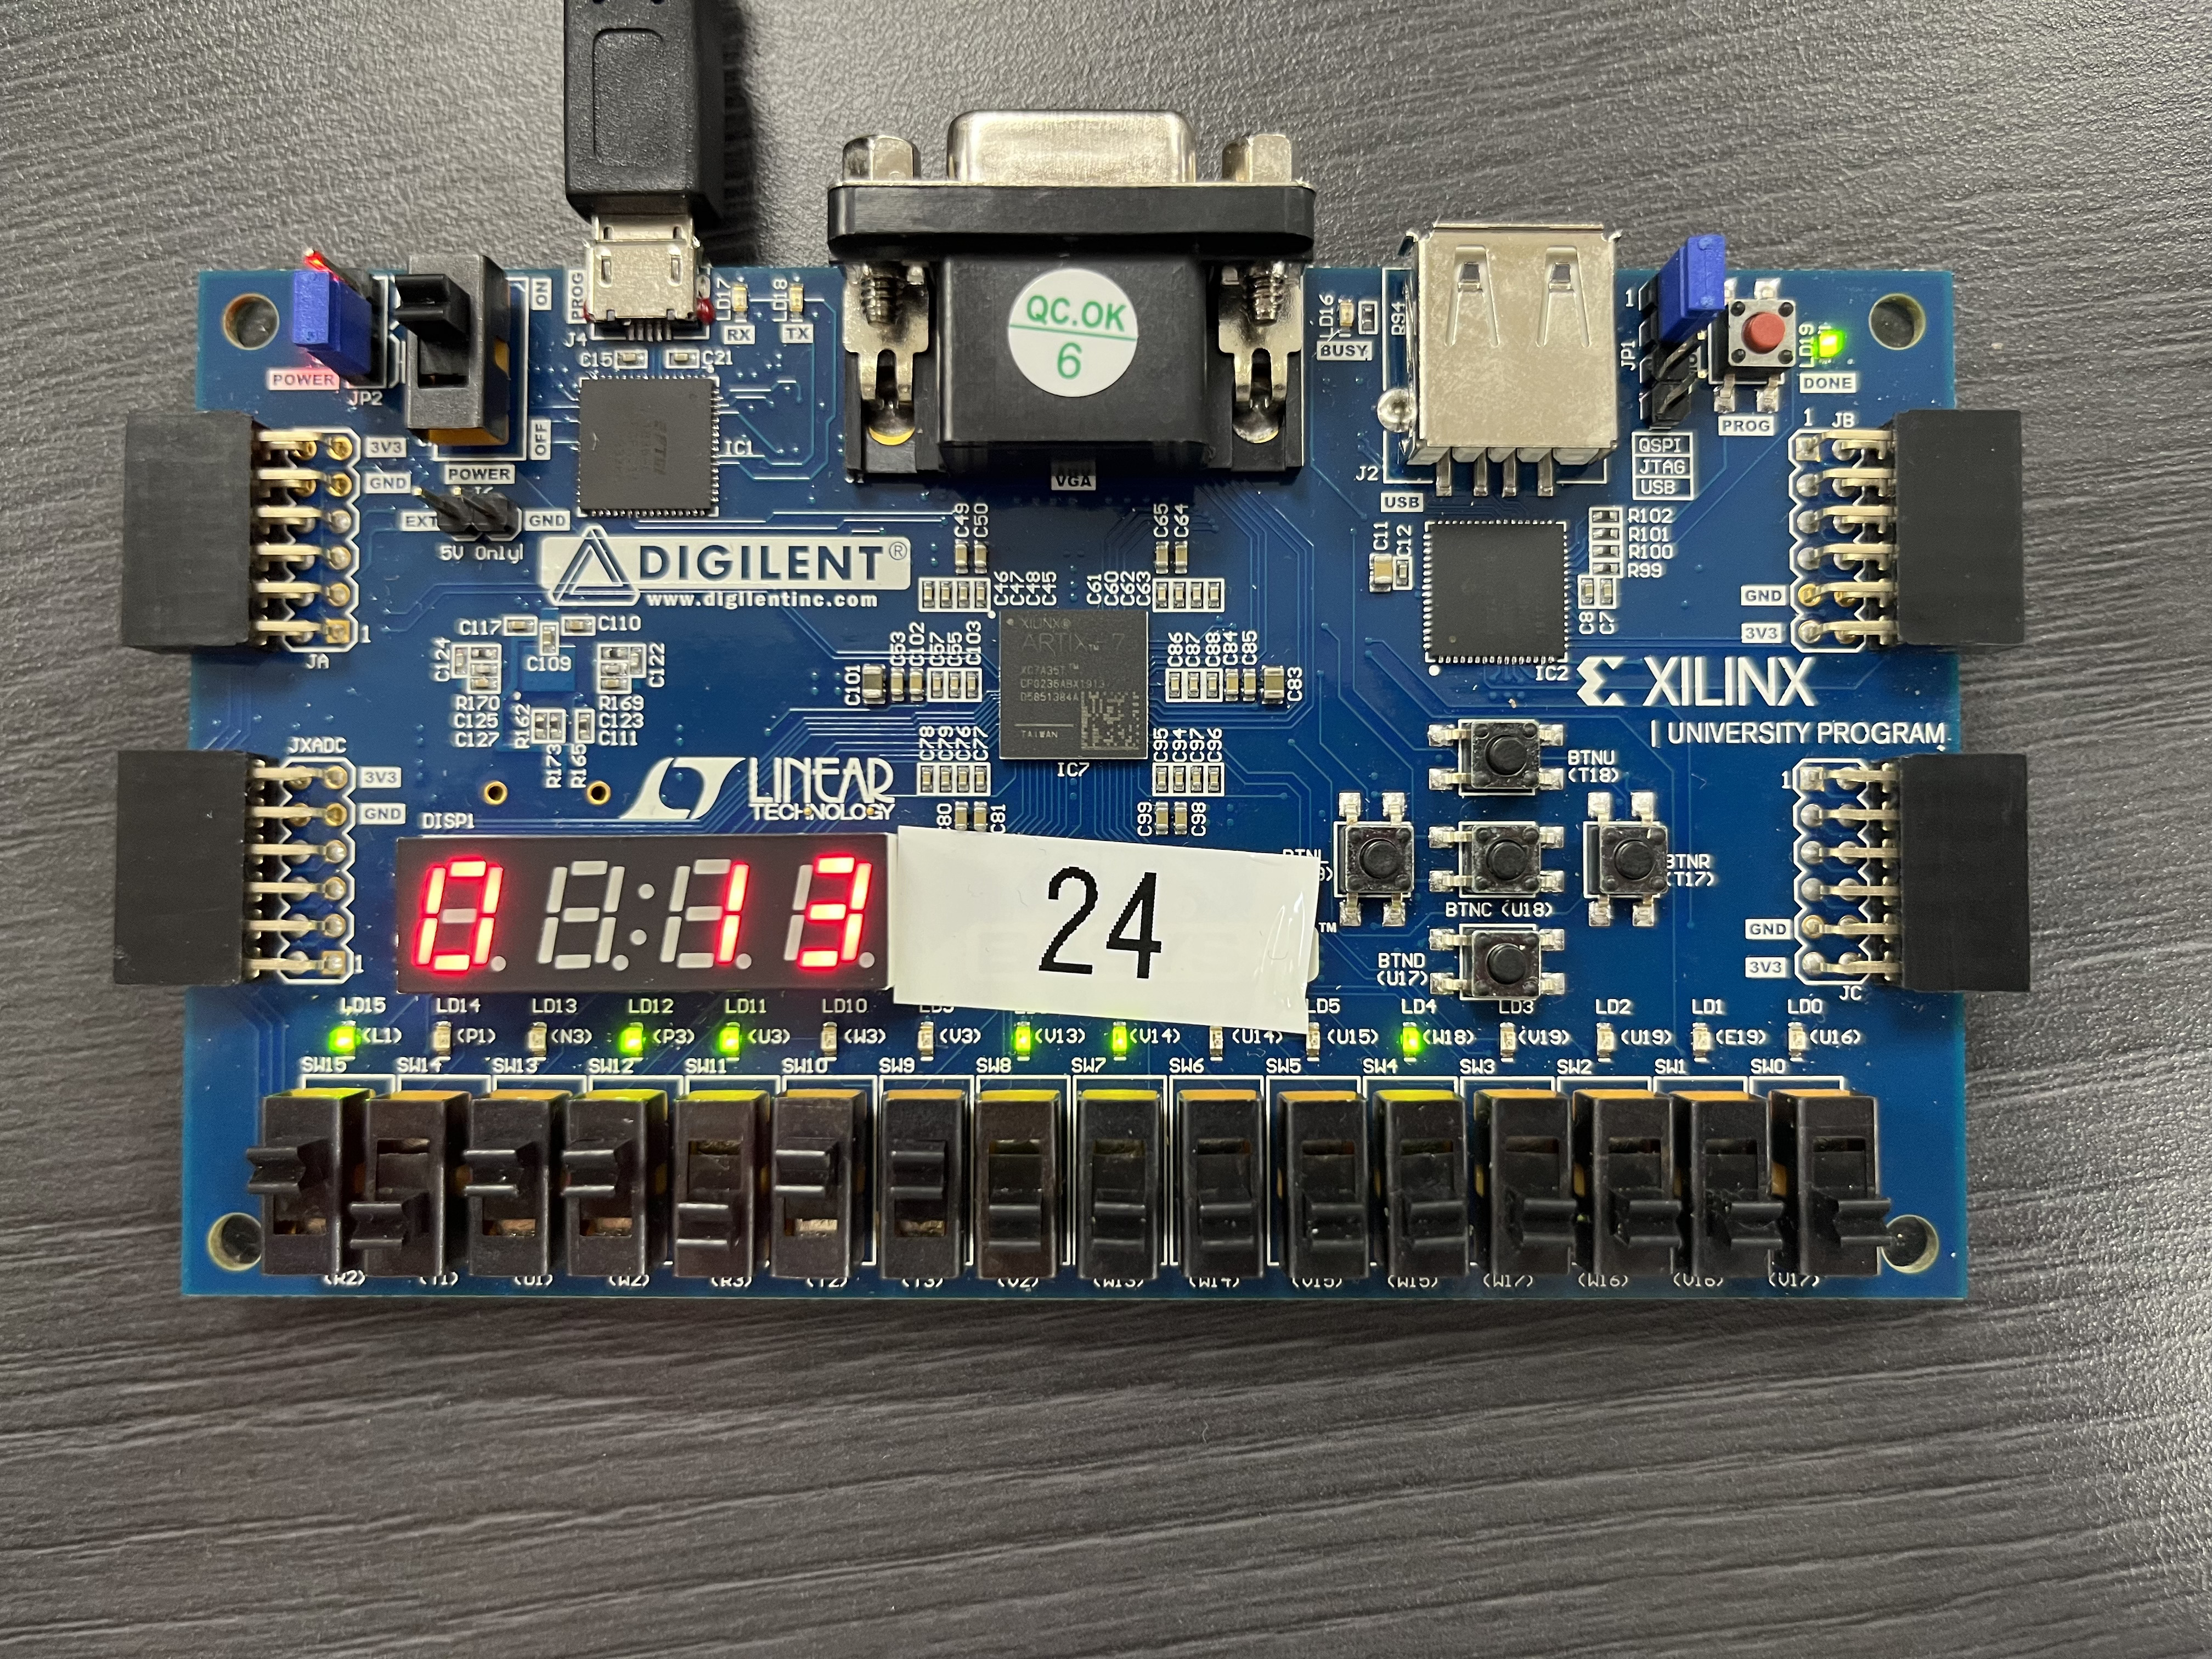
\includegraphics[width=1\linewidth]{sel0_13_06.jpg}
    \caption{\texttt{sel = 0}}
  \end{minipage}\quad
  \begin{minipage}{0.45\linewidth}
    \centering
    \includegraphics[width=1\linewidth]{sel1_13_06.jpg}
    \caption{\texttt{sel = 1}}
  \end{minipage}
\end{figure}
\begin{figure}[H]
  \centering
  \begin{minipage}{0.45\linewidth}
    \centering
    \includegraphics[width=1\linewidth]{sel2_13_06.jpg}
    \caption{\texttt{sel = 2}}
  \end{minipage}\quad
  \begin{minipage}{0.45\linewidth}
    \centering
    \includegraphics[width=1\linewidth]{sel3_13_06.jpg}
    \caption{\texttt{sel = 3}}
  \end{minipage}
\end{figure}
\begin{figure}[H]
  \centering
  \begin{minipage}{0.45\linewidth}
    \centering
    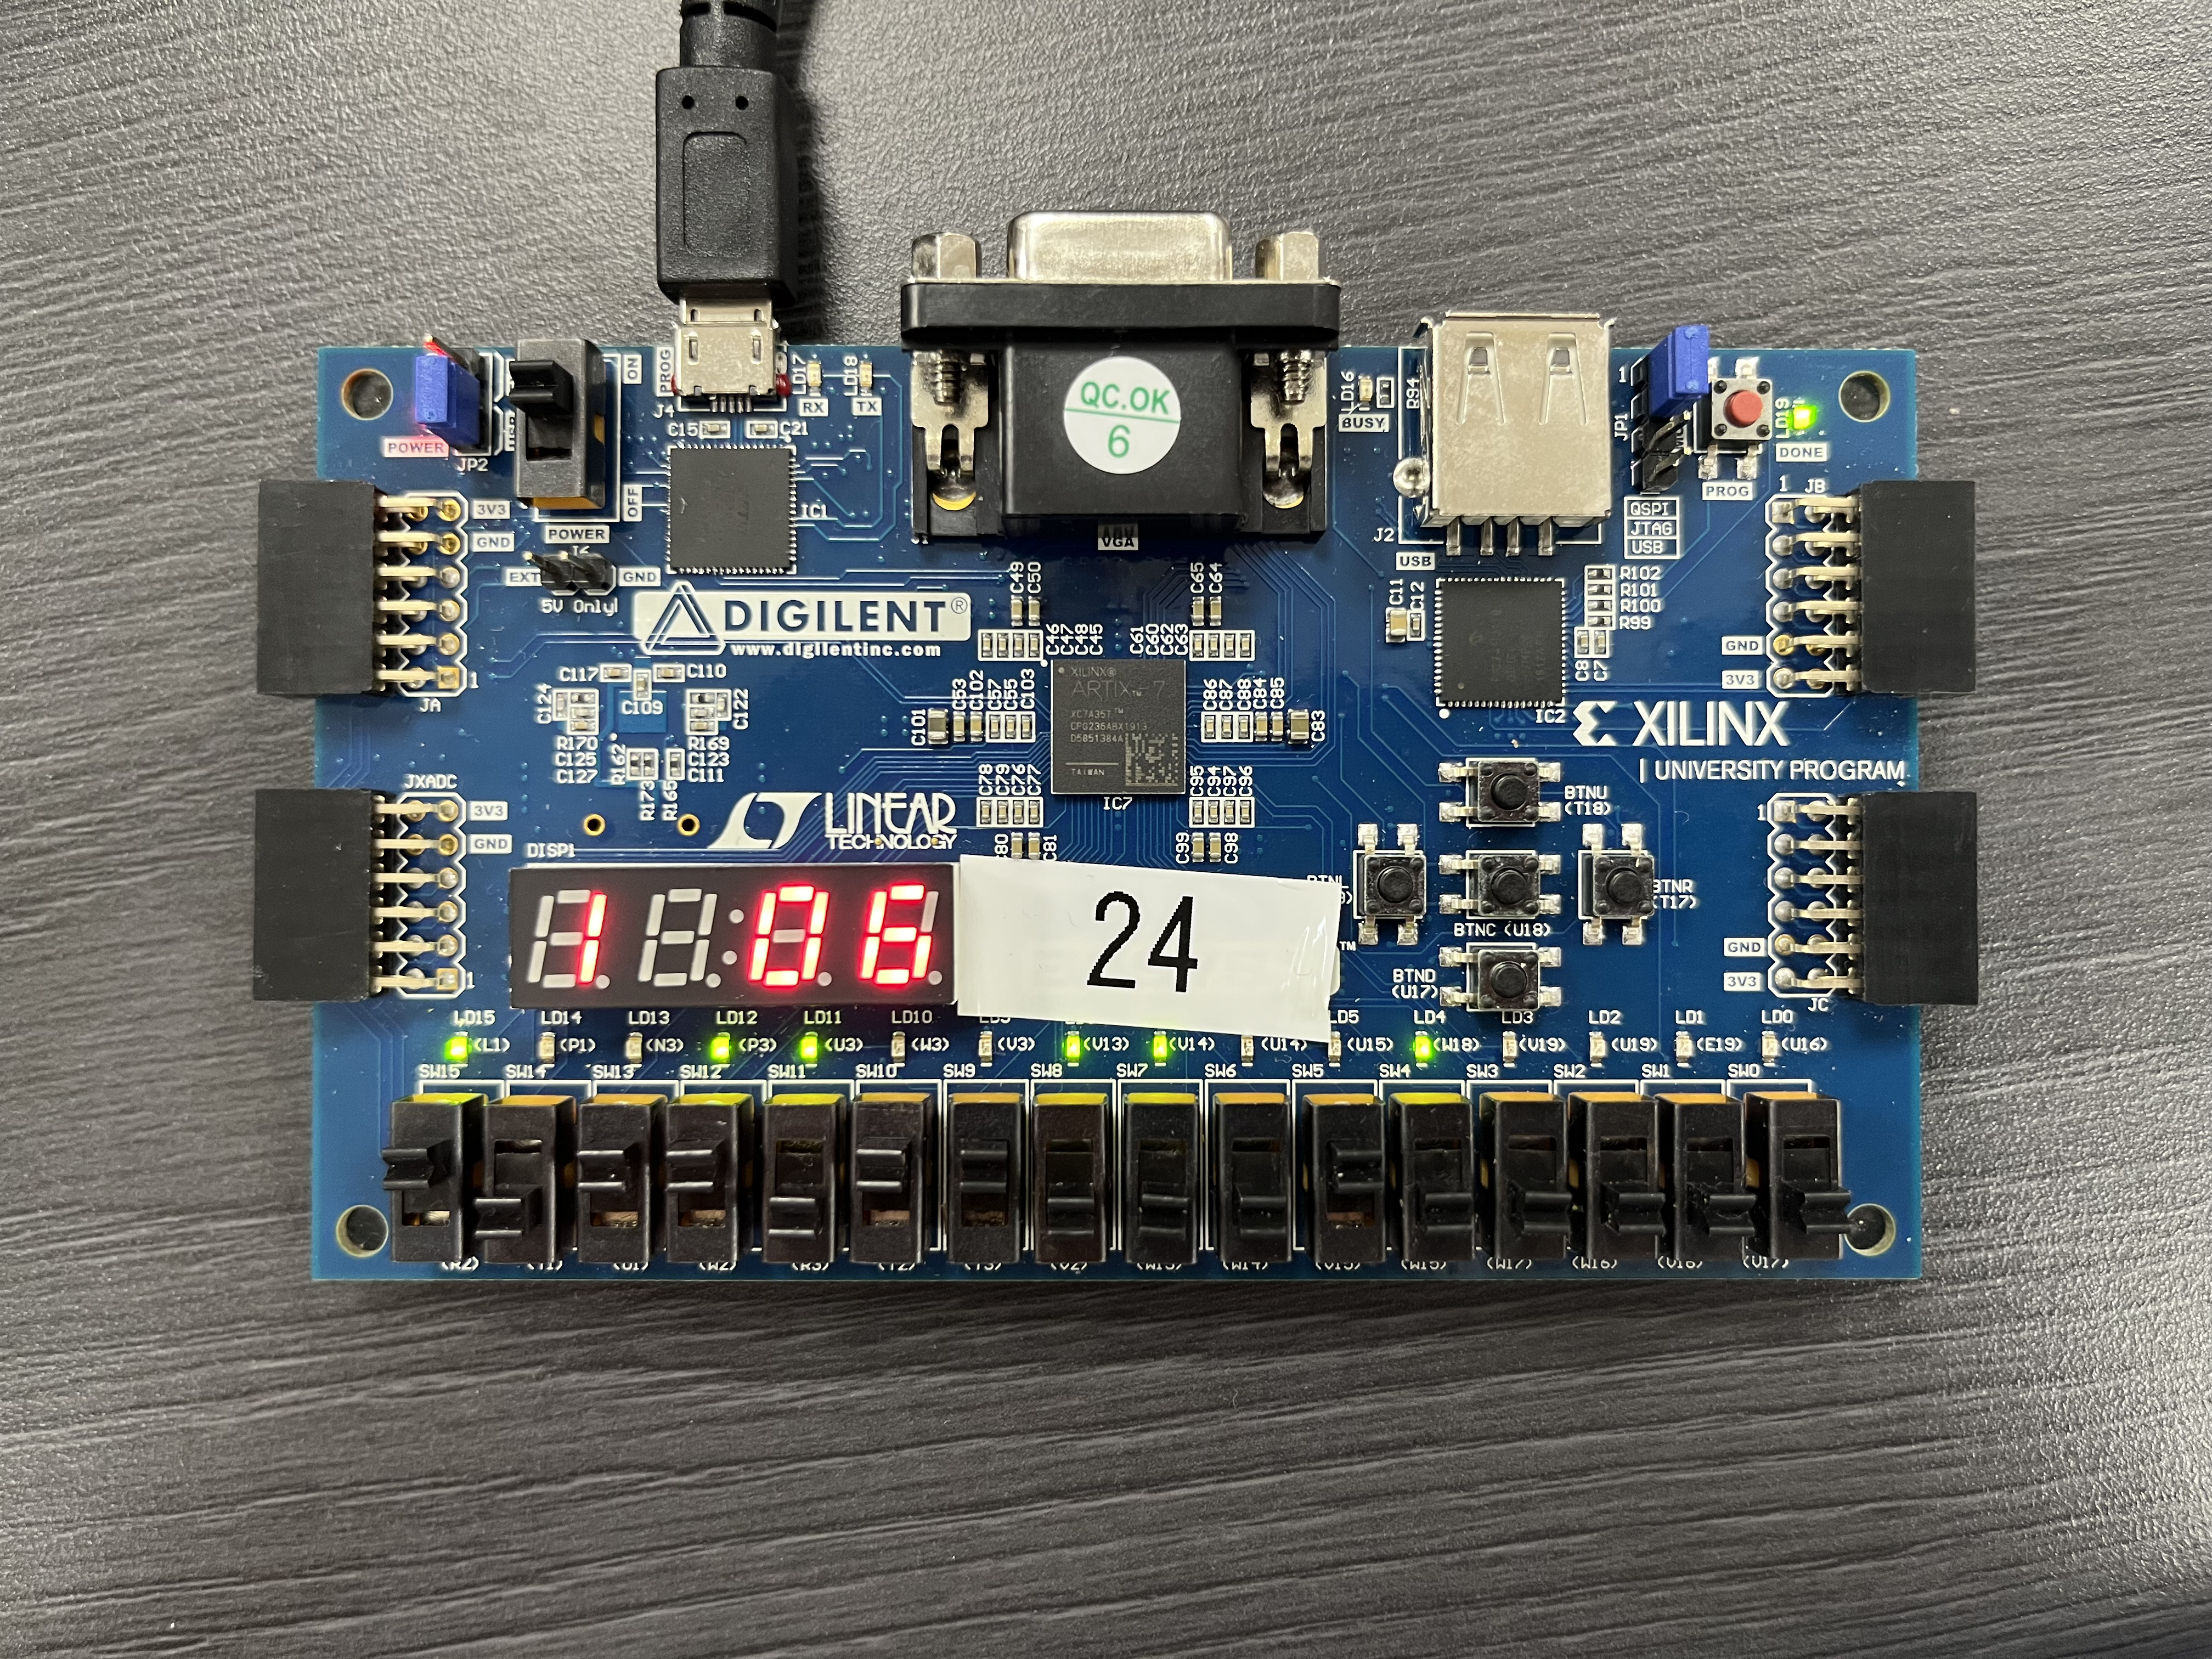
\includegraphics[width=1\linewidth]{sel4_13_06.jpg}
    \caption{\texttt{sel = 4}}
  \end{minipage}\quad
  \begin{minipage}{0.45\linewidth}
    \centering
    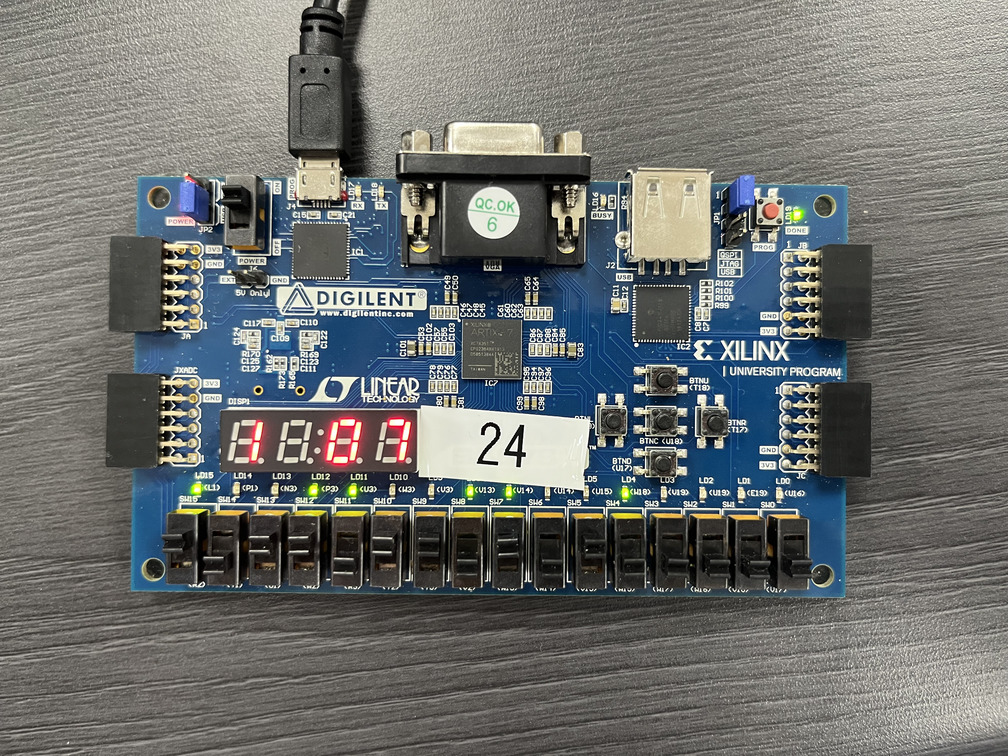
\includegraphics[width=1\linewidth]{sel5_13_06.jpg}
    \caption{\texttt{sel = 5}}
  \end{minipage}
\end{figure}
\begin{figure}[H]
  \centering
  \begin{minipage}{0.45\linewidth}
    \centering
    \includegraphics[width=1\linewidth]{sel6_13_06.jpg}
    \caption{\texttt{sel = 6}}
  \end{minipage}\quad
  \begin{minipage}{0.45\linewidth}
    \centering
    \includegraphics[width=1\linewidth]{sel7_13_06.jpg}
    \caption{\texttt{sel = 7}}
  \end{minipage}
\end{figure}
\begin{figure}[H]
  \centering
  \begin{minipage}{0.45\linewidth}
    \centering
    \includegraphics[width=1\linewidth]{sel8_13_06.jpg}
    \caption{\texttt{sel = 8}}
  \end{minipage}\quad
  \begin{minipage}{0.45\linewidth}
    \centering
    \includegraphics[width=1\linewidth]{sel9_13_06.jpg}
    \caption{\texttt{sel = 9}}
  \end{minipage}
\end{figure}
\begin{figure}[H]
  \centering
  \begin{minipage}{0.45\linewidth}
    \centering
    \includegraphics[width=1\linewidth]{sel10_13_06.jpg}
    \caption{\texttt{sel = 10}}
  \end{minipage}\quad
  \begin{minipage}{0.45\linewidth}
    \centering
    \includegraphics[width=1\linewidth]{sel11_13_06.jpg}
    \caption{\texttt{sel = 11}}
  \end{minipage}
\end{figure}

\subsection{\texttt{lab5\_2.v} -- Negative Reset Master-Slave JK Flip-Flop}
SR latch 두 개를 연결한 회로도는 다음과 같다.
\begin{figure}[H]
  \centering
  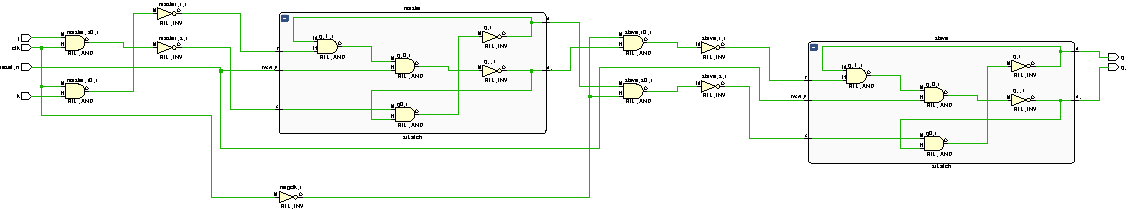
\includegraphics[width=0.9\linewidth]{lab5_2_simple_schematic-crop.pdf}
\end{figure}
테스트벤치 실행 결과 다음 파형을 얻을 수 있었다.
\begin{figure}[H]
  \centering
  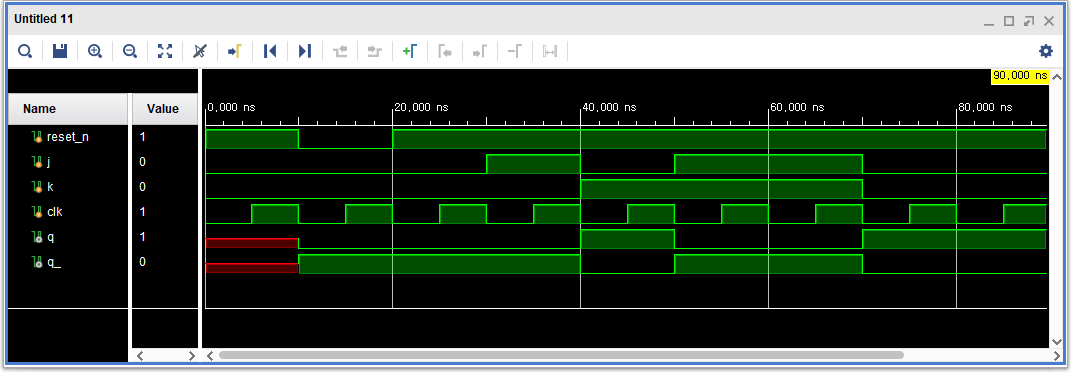
\includegraphics[width=0.9\linewidth]{lab5_2_simple_waveform.png}
\end{figure}
50ns 지점부터 20ns 동안 \(J = K = 1\) 입력이 주어졌지만 toggle이 작동하지 않는 모습을 볼 수 있다.
또한, 이 회로에서는 짧은 시간동안 1이 입력되었을 때 출력에 영향을 미치는 1's catch 현상이 일어난다.
\begin{figure}[H]
  \centering
  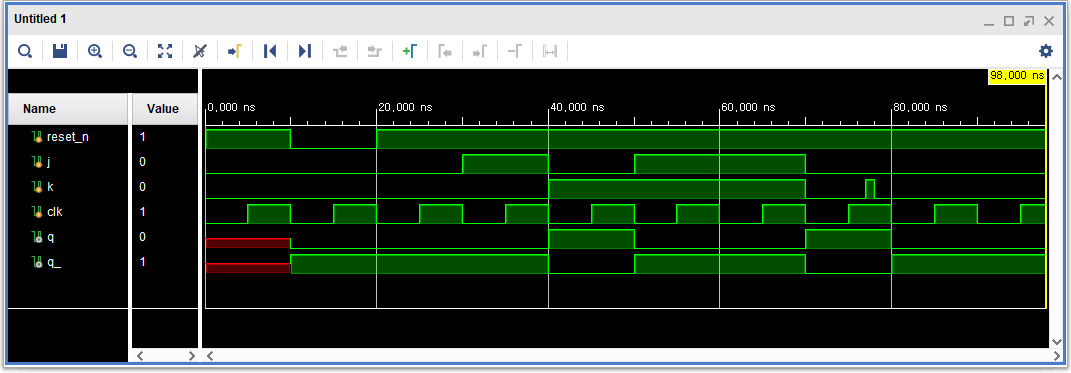
\includegraphics[width=0.9\linewidth]{lab5_2_simple_1catch_waveform.png}
\end{figure}
1ns 동안 잠시 \(K = 1\) 입력이 주어졌을 때, 출력이 바뀌는 것을 볼 수 있다.

Negative reset master-slave JK flip-flop을 구현한 회로도는 다음과 같다.
\begin{figure}[H]
  \centering
  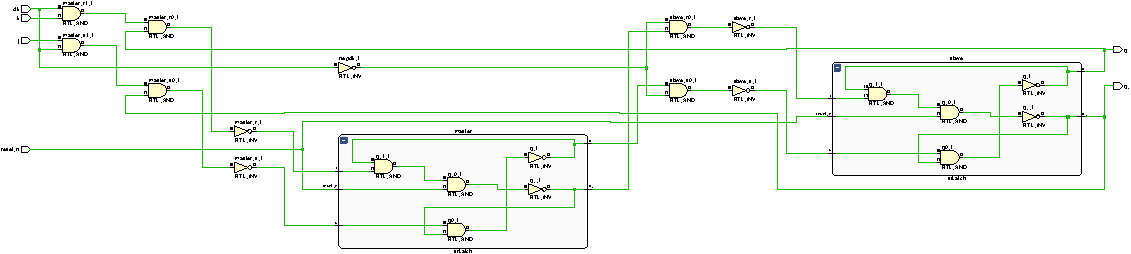
\includegraphics[width=0.9\linewidth]{lab5_2_schematic-crop.pdf}
\end{figure}
테스트벤치 실행 결과 파형은 다음과 같다.
\begin{figure}[H]
  \centering
  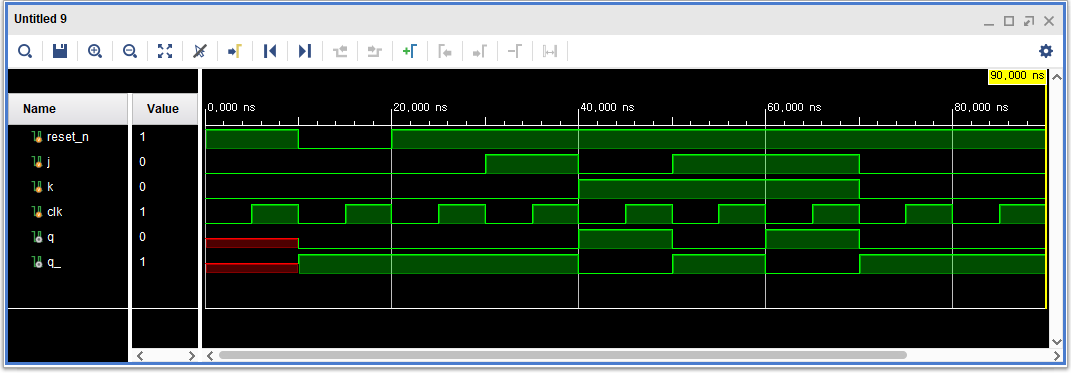
\includegraphics[width=0.9\linewidth]{lab5_2_fixed_waveform.png}
\end{figure}
단순히 SR latch 두 개를 연결했을 때와 달리, toggle이 작동하는 것을 볼 수 있다.
한편, 이 회로에서도 1's catch 현상은 일어난다. 1ns 동안 잠시 \(J = 1\) 입력이 주어졌을 때 출력이 바뀌었다.
\begin{figure}[H]
  \centering
  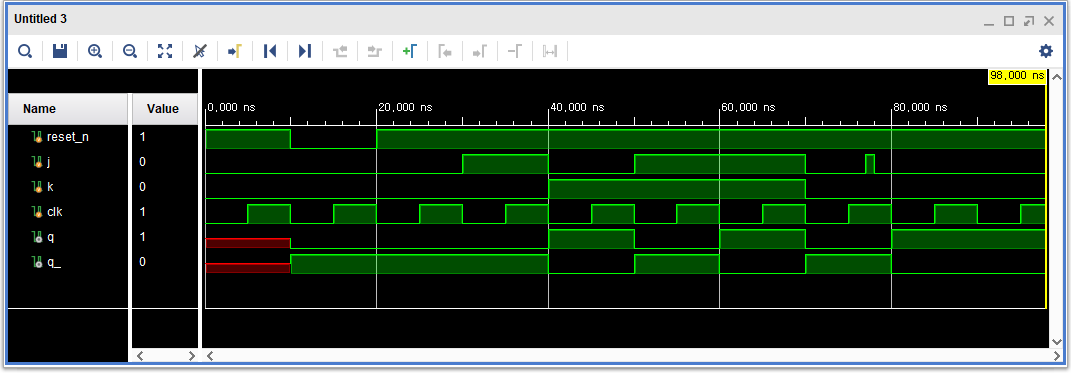
\includegraphics[width=0.9\linewidth]{lab5_2_fixed_1catch_waveform.png}
\end{figure}

\section{논의}
ALU와 flip-flop을 구현하면서 컴퓨터의 구조에 대해 알 수 있는 시간이었다.
구현과 실험 등에서 몇 가지 시행착오를 거쳤지만 지금까지 배운 내용으로 실제 동작하는 회로를 만들었다는 사실이 뜻깊었다.

\end{document}
